\section{Multi-Index Monte Carlo}

\begin{frame}
	\frametitle{Erweiterung: Multi-Index Monte Carlo\footnote{Weiterf. Informationen in \glqq Multi index Monte Carlo: when sparsity meets sampling\grqq\ von Haji-Ali et al. (2014)}}
	\textbf{Idee:} Mehrdimensionale Levelindizes
	\newline
	$\Rightarrow$ Ermöglicht bspw. unterschiedliche Diskretisierungsweiten in \noindent\hspace*{5mm}unterschiedliche Koordinatenrichtungen.
	\begin{figure}[H]
		\centering
		\begin{adjustbox}{width=0.4\paperwidth, center}
			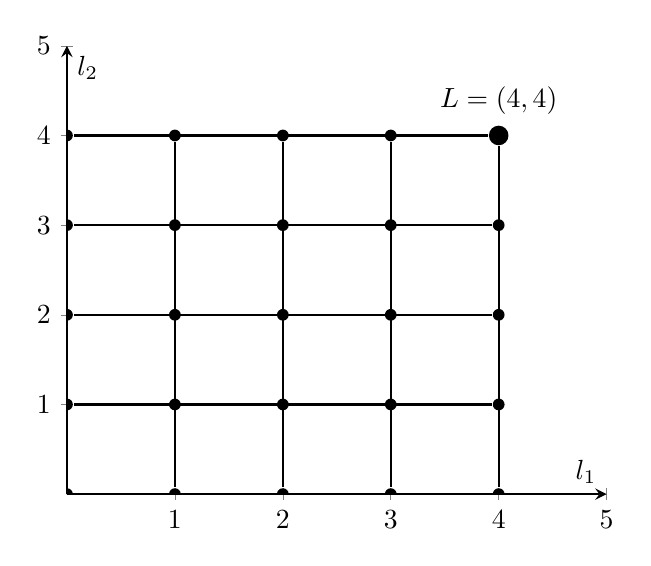
\begin{tikzpicture}
				\begin{axis} [ 
					style=thick, 
					xlabel=$l_1$,
					ylabel=$l_2$,
					minor tick num=0, 
					xmin=0, xmax=5,  
					ymin=0, ymax=5,
					axis x line=middle,
					axis y line=middle,
					xtick={0,1,...,5},
					ytick={0,1,...,5}
				  ]
					\node[circle,fill,inner sep=1.5pt] (P11) at (axis cs:1,1) {};
					\node[circle,fill,inner sep=1.5pt] (P12) at (axis cs:1,2) {};
					\node[circle,fill,inner sep=1.5pt] (P21) at (axis cs:2,1) {};
					\node[circle,fill,inner sep=1.5pt] (P22) at (axis cs:2,2) {};
					\node[circle,fill,inner sep=1.5pt] (P31) at (axis cs:3,1) {};
					\node[circle,fill,inner sep=1.5pt] (P32) at (axis cs:3,2) {};
					\node[circle,fill,inner sep=1.5pt] (P33) at (axis cs:3,3) {};
					\node[circle,fill,inner sep=1.5pt] (P13) at (axis cs:1,3) {};
					\node[circle,fill,inner sep=1.5pt] (P23) at (axis cs:2,3) {};
					\node[circle,fill,inner sep=1.5pt] (P41) at (axis cs:4,1) {};
					\node[circle,fill,inner sep=1.5pt] (P42) at (axis cs:4,2) {};
					\node[circle,fill,inner sep=1.5pt] (P43) at (axis cs:4,3) {};
					\node[label={$L=(4,4)$},circle,fill,inner sep=2.5pt] (P44) at (axis cs:4,4) {};
					\node[circle,fill,inner sep=1.5pt] (P14) at (axis cs:1,4) {};
					\node[circle,fill,inner sep=1.5pt] (P24) at (axis cs:2,4) {};
					\node[circle,fill,inner sep=1.5pt] (P34) at (axis cs:3,4) {};
					\node[circle,fill,inner sep=1.5pt] (P01) at (axis cs:0,1) {};
					\node[circle,fill,inner sep=1.5pt] (P02) at (axis cs:0,2) {};
					\node[circle,fill,inner sep=1.5pt] (P03) at (axis cs:0,3) {};
					\node[circle,fill,inner sep=1.5pt] (P04) at (axis cs:0,4) {};
					\node[circle,fill,inner sep=1.5pt] (P10) at (axis cs:1,0) {};
					\node[circle,fill,inner sep=1.5pt] (P20) at (axis cs:2,0) {};
					\node[circle,fill,inner sep=1.5pt] (P30) at (axis cs:3,0) {};
					\node[circle,fill,inner sep=1.5pt] (P40) at (axis cs:4,0) {};
					\node[circle,fill,inner sep=1.5pt] (P00) at (axis cs:0,0) {};
					\draw [-] (P03) to (P43);
					\draw [-] (P30) to (P34);
					\draw [-] (P02) to (P42);
					\draw [-] (P20) to (P24);
					\draw [-] (P40) to (P44);
					\draw [-] (P04) to (P44);
					\draw [-] (P01) to (P41);
					\draw [-] (P10) to (P14);
				\end{axis} 
			\end{tikzpicture}
		\end{adjustbox}
		\caption{Zwei-dimensionale Indizes}
		\label{}
	\end{figure}
\end{frame}

\begin{frame}
	\frametitle{Multilevel Teleskopsumme im Mehrdimensionalen}
	Wir definieren für $l=(l_i)_{i=1}^d\in\mathbb{N}^d$ die Differenz
	\[
		\Delta_iP_l=\begin{cases}
		P_l-P_{l-e_i}, & l_i>0\\P_l, & l_i=0
		\end{cases}
	\]
	wobei $e_i$ den Einheitsvektor in Koordinatenrichtung $i$ bezeichnet.
	\onslide<2->{
	\newline
	Sei zudem
	\[
		\Delta P_l=\left(\prod\limits_{i=1}^d\Delta_i\right)P_l.
	\]
	}
	\onslide<3->{
	\newline
	Es ergibt sich mit $I=\{l\in\mathbb{N}^d:l\geq 0\}$ der Schätzer
	\[
		Y:=\sum\limits_{l\in I}\mathbb{E}[\Delta P_l]
	\]
	für $\mathbb{E}[P]$.
	}
\end{frame}

\begin{frame}
	\frametitle{Beispiel: Natürliche Wahl von $I$}
	Sei
	\[
		I=\left\{(l_1,l_2)\in\mathbb{N}^2:0\leq l_1\leq 3\ \text{und}\ 0\leq l_2\leq 2\right\}.
	\]
	\onslide<2->{
	$I$ entspricht nun einem Rechteck mit Eckpunkt $(3,2)$.
	\begin{figure}[H]
		\centering
		\begin{adjustbox}{width=0.35\paperwidth, center}
			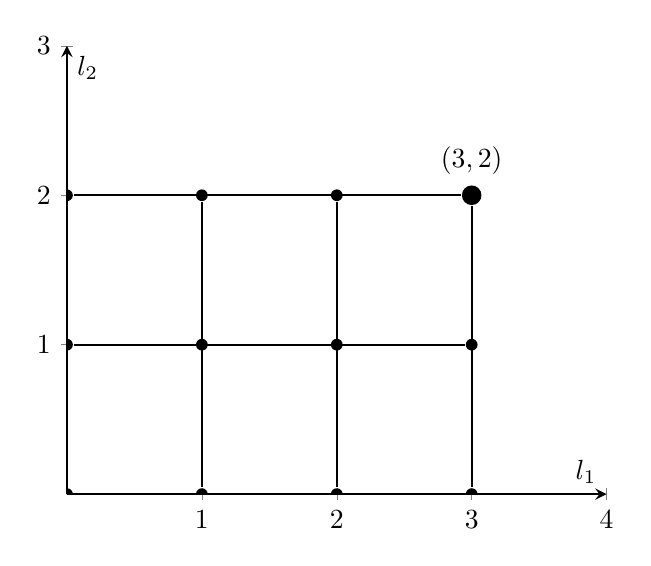
\begin{tikzpicture} 
				\begin{axis} [ 
					style=thick, 
					xlabel=$l_1$,
					ylabel=$l_2$,
					minor tick num=0, 
					xmin=0, xmax=4,  
					ymin=0, ymax=3,
					axis x line=middle,
					axis y line=middle,
					xtick={0,1,...,4},
					ytick={0,1,...,3}
				  ]
					\node[circle,fill,inner sep=1.5pt] (P11) at (axis cs:1,1) {};
					\node[circle,fill,inner sep=1.5pt] (P12) at (axis cs:1,2) {};
					\node[circle,fill,inner sep=1.5pt] (P21) at (axis cs:2,1) {};
					\node[circle,fill,inner sep=1.5pt] (P22) at (axis cs:2,2) {};
					\node[circle,fill,inner sep=1.5pt] (P31) at (axis cs:3,1) {};
					\node[label={$(3,2)$},circle,fill,inner sep=2.5pt] (P32) at (axis cs:3,2) {};
					\node[circle,fill,inner sep=1.5pt] (P01) at (axis cs:0,1) {};
					\node[circle,fill,inner sep=1.5pt] (P02) at (axis cs:0,2) {};
					\node[circle,fill,inner sep=1.5pt] (P30) at (axis cs:3,0) {};
					\node[circle,fill,inner sep=1.5pt] (P10) at (axis cs:1,0) {};
					\node[circle,fill,inner sep=1.5pt] (P20) at (axis cs:2,0) {};
					\node[circle,fill,inner sep=1.5pt] (P00) at (axis cs:0,0) {};
					\draw [-] (P02) to (P32);
					\draw [-] (P30) to (P32);
					\draw [-] (P20) to (P22);
					\draw [-] (P01) to (P31);
					\draw [-] (P10) to (P12);
				\end{axis} 
			\end{tikzpicture}
		\end{adjustbox}
	\end{figure}
	Dann ist $\Delta P_{(3,2)}=\Delta_1\Delta_2 P_{(3,2)}=P_{(3,2)}-P_{(2,2)}-P_{(3,1)}+P_{(2,1)}$ und $Y=\mathbb{E}[P_{(3,2)}]$.
	}
\end{frame}

\begin{frame}[t]
	\frametitle{Wie sollte $I$ gewählt werden?}
	Die optimale Wahl ist (ähnlich zu dünnen Gittern)
	\[
		I=\{l\in\mathbb{N}^d:l\geq 0,\ \langle l,n\rangle\leq L\}
	\]
	für eine Richtung $n\in\mathbb{N}^d,n>0,$ und ein $L\in\mathbb{N}$.
	\begin{figure}[H]
		\only<2->{
		\centering
		\begin{adjustbox}{height=0.46\paperheight, center}
			\begin{tikzpicture} 
				\begin{axis} [ 
					style=thick,
					xlabel=$l_1$,
					ylabel=$l_2$,
					minor tick num=0,
					xmin=0, xmax=7,
					ymin=1, ymax=4,
					axis x line=middle,
					axis y line=middle,
					xtick={0,1,...,7},
					ytick={0,1,...,4},
					axis equal
				  ]
					\node[circle,fill,inner sep=1.5pt] (P11) at (axis cs:1,1) {};
					\node[circle,fill,inner sep=1.5pt] (P12) at (axis cs:1,2) {};
					\node[circle,fill,inner sep=1.5pt] (P21) at (axis cs:2,1) {};
					\node[circle,fill,inner sep=1.5pt] (P22) at (axis cs:2,2) {};
					\node[circle,fill,inner sep=1.5pt] (P31) at (axis cs:3,1) {};
					\node[circle,fill,inner sep=1.5pt] (P01) at (axis cs:0,1) {};
					\node[circle,fill,inner sep=1.5pt] (P02) at (axis cs:0,2) {};
					\node[circle,fill,inner sep=1.5pt] (P03) at (axis cs:0,3) {};
					\node[circle,fill,inner sep=1.5pt] (P10) at (axis cs:1,0) {};
					\node[circle,fill,inner sep=1.5pt] (P20) at (axis cs:2,0) {};
					\node[circle,fill,inner sep=1.5pt] (P30) at (axis cs:3,0) {};
					\node[circle,fill,inner sep=1.5pt] (P40) at (axis cs:4,0) {};
					\node[circle,fill,inner sep=1.5pt] (P50) at (axis cs:5,0) {};
					\node[circle,fill,inner sep=1.5pt] (P60) at (axis cs:6,0) {};
					\node[circle,fill,inner sep=1.5pt] (P41) at (axis cs:4,1) {};
					\node[circle,fill,inner sep=1.5pt] (P00) at (axis cs:0,0) {};
					\draw [-] (P60) to (P03);
					\draw [-] (P30) to (P31);
					\draw [-] (P20) to (P22);
					\draw [-] (P02) to (P22);
					\draw [-] (P01) to (P41);
					\draw [-] (P10) to (P12);
					\draw [-] (P40) to (P41);
					\draw [-] (P50) to (axis cs:5,0.5);
					\draw [-] (P31) to (axis cs:3,1.5);
					\draw [-] (P12) to (axis cs:1,2.5);
					\only<3->{
						\node (N) at (axis cs:4,3.5) {};
						\draw [->,color=red, line width=1pt] (axis cs:3,1.5) to (N) node [below right] {$\bm{n}$};
						\node (TEMP) at (axis cs:3,1.5) {};
						\pic[draw=black,angle eccentricity=0.5,angle radius=.5cm, color=red, line width=1pt, pic text={$\bm{\cdot}$}]
						{angle=N--TEMP--P22};
					}
				\end{axis} 
			\end{tikzpicture}
		\end{adjustbox}
		\caption{Beispiel mit $L=6$ und $n=[1,2]^T$}
	}
	\end{figure}

	
%	\begin{figure}[H]
%		\centering
%		\begin{adjustbox}{width=0.4\paperwidth, center}
%			\begin{tikzpicture} 
%				\begin{axis} [ 
%					style=thick, 
%					xlabel=$l_1$,
%					ylabel=$l_2$,
%					minor tick num=0, 
%					xmin=0, xmax=5,  
%					ymin=0, ymax=5,
%					axis x line=middle,
%					axis y line=middle,
%					xtick={0,1,...,5},
%					ytick={0,1,...,5}
%				  ]
%					\node[circle,fill,inner sep=1.5pt] (P11) at (axis cs:1,1) {};
%					\node[circle,fill,inner sep=1.5pt] (P12) at (axis cs:1,2) {};
%					\node[circle,fill,inner sep=1.5pt] (P21) at (axis cs:2,1) {};
%					\node[circle,fill,inner sep=1.5pt] (P22) at (axis cs:2,2) {};
%					\node[circle,fill,inner sep=1.5pt] (P31) at (axis cs:3,1) {};
%					\node[circle,fill,inner sep=1.5pt] (P13) at (axis cs:1,3) {};
%					\node[circle,fill,inner sep=1.5pt] (P01) at (axis cs:0,1) {};
%					\node[circle,fill,inner sep=1.5pt] (P02) at (axis cs:0,2) {};
%					\node[circle,fill,inner sep=1.5pt] (P03) at (axis cs:0,3) {};
%					\node[circle,fill,inner sep=1.5pt] (P04) at (axis cs:0,4) {};
%					\node[circle,fill,inner sep=1.5pt] (P10) at (axis cs:1,0) {};
%					\node[circle,fill,inner sep=1.5pt] (P20) at (axis cs:2,0) {};
%					\node[circle,fill,inner sep=1.5pt] (P30) at (axis cs:3,0) {};
%					\node[circle,fill,inner sep=1.5pt] (P40) at (axis cs:4,0) {};
%					\node[circle,fill,inner sep=1.5pt] (P00) at (axis cs:0,0) {};
%					\draw [-] (P40) to (P04);
%					\draw [-] (P03) to (P13);
%					\draw [-] (P30) to (P31);
%					\draw [-] (P20) to (P22);
%					\draw [-] (P02) to (P22);
%					\draw [-] (P01) to (P31);
%					\draw [-] (P10) to (P13);
%				\end{axis} 
%			\end{tikzpicture}
%		\end{adjustbox}
%		\caption{Beispiel für $L=4$ und $n=[1,1]^T$}
%		\label{}
%	\end{figure}
\end{frame}

\begin{frame}[c]
	\frametitle{Optimale Wahl von $I$ in 3D}
	\tdplotsetmaincoords{70}{110}
	\begin{figure}[H]
		\centering
		\begin{adjustbox}{width=0.49\paperwidth, center}
			\begin{tikzpicture}[tdplot_main_coords]
				\coordinate[circle,fill,inner sep=1.5pt] (P112) at (1,1,2);
				\coordinate[circle,fill,inner sep=1.5pt] (P121) at (1,2,1);
				\coordinate[circle,fill,inner sep=1.5pt] (P211) at (2,1,1);
				\coordinate[circle,fill,inner sep=1.5pt] (P111) at (1,1,1);
				\coordinate[circle,fill,inner sep=1.5pt] (P021) at (0,2,1);
				\coordinate[circle,fill,inner sep=1.5pt] (P031) at (0,3,1);
				\coordinate[circle,fill,inner sep=1.5pt] (P011) at (0,1,1);
				\coordinate[circle,fill,inner sep=1.5pt] (P012) at (0,1,2);
				\coordinate[circle,fill,inner sep=1.5pt] (P022) at (0,2,2);
				\coordinate[circle,fill,inner sep=1.5pt] (P013) at (0,1,3);
				\coordinate[circle,fill,inner sep=1.5pt] (P040) at (0,4,0);
				\coordinate[circle,fill,inner sep=1.5pt] (P004) at (0,0,4);
				\coordinate[circle,fill,inner sep=1.5pt] (P030) at (0,3,0);
				\coordinate[circle,fill,inner sep=1.5pt] (P130) at (1,3,0);
				\coordinate[circle,fill,inner sep=1.5pt] (P020) at (0,2,0);
				\coordinate[circle,fill,inner sep=1.5pt] (P120) at (1,2,0);
				\coordinate[circle,fill,inner sep=1.5pt] (P220) at (2,2,0);
				\coordinate[circle,fill,inner sep=1.5pt] (P010) at (0,1,0);
				\coordinate[circle,fill,inner sep=1.5pt] (P110) at (1,1,0);
				\coordinate[circle,fill,inner sep=1.5pt] (P210) at (2,1,0);
				\coordinate[circle,fill,inner sep=1.5pt] (P310) at (3,1,0);
				\coordinate[circle,fill,inner sep=1.5pt] (P003) at (0,0,3);
				\coordinate[circle,fill,inner sep=1.5pt] (P103) at (1,0,3);
				\coordinate[circle,fill,inner sep=1.5pt] (P002) at (0,0,2);
				\coordinate[circle,fill,inner sep=1.5pt] (P102) at (1,0,2);
				\coordinate[circle,fill,inner sep=1.5pt] (P202) at (2,0,2);
				\coordinate[circle,fill,inner sep=1.5pt] (P001) at (0,0,1);
				\coordinate[circle,fill,inner sep=1.5pt] (P101) at (1,0,1);
				\coordinate[circle,fill,inner sep=1.5pt] (P201) at (2,0,1);
				\coordinate[circle,fill,inner sep=1.5pt] (P301) at (3,0,1);
				\coordinate[circle,fill,inner sep=1.5pt] (P100) at (1,0,0);
				\coordinate[circle,fill,inner sep=1.5pt] (P200) at (2,0,0);
				\coordinate[circle,fill,inner sep=1.5pt] (P300) at (3,0,0);
				\coordinate[circle,fill,inner sep=1.5pt] (P400) at (4,0,0);
				\coordinate[circle,fill,inner sep=1.5pt] (P000) at (0,0,0);
				\draw[->] (0,0,0) -- (5,0,0) node[anchor=north east]{$l_1$};
				\draw[->] (0,0,0) -- (0,5,0) node[anchor=north west]{$l_2$};
				\draw[->] (0,0,0) -- (0,0,5) node[anchor=south]{$l_3$};

				\draw[-] (P400) -- (P040) -- (P004) -- (P400);

				\draw[-] (P100) -- (P130);
				\draw[-] (P130) -- (P030);
				\draw[-] (P200) -- (P220);
				\draw[-] (P220) -- (P020);
				\draw[-] (P300) -- (P310);
				\draw[-] (P310) -- (P010);
				\draw[-] (P101) -- (P121);
				\draw[-] (P121) -- (P021);
				\draw[-] (P201) -- (P211);
				\draw[-] (P211) -- (P011);
				\draw[-] (P001) -- (P301);
				\draw[-] (P001) -- (P031);
				\draw[-] (P301) -- (P031);
				\draw[-] (P002) -- (P202);
				\draw[-] (P002) -- (P022);
				\draw[-] (P102) -- (P112);
				\draw[-] (P112) -- (P012);
				\draw[-] (P202) -- (P022);
				\draw[-] (P103) -- (P013);
				\draw[-] (P003) -- (P103);
				\draw[-] (P003) -- (P013);
				\draw[-] (P130) -- (P030);
				\draw[-] (P100) -- (P103);
				\draw[-] (P200) -- (P202);
				\draw[-] (P130) -- (P030);
				\draw[-] (P300) -- (P301);
				\draw[-] (P110) -- (P112);
				\draw[-] (P210) -- (P211);
				\draw[-] (P120) -- (P121);
				\draw[-] (P010) -- (P013);
				\draw[-] (P020) -- (P022);
				\draw[-] (P030) -- (P031);
			\end{tikzpicture}
		\end{adjustbox}
		\caption{Beispiel mit $L=4$ und $n=[1,1,1]^T$}
		\label{}
	\end{figure}
\end{frame}